\chapter{Fundamentos y modelo causal}\label{cap:marco}

\section{Resultados potenciales y estimando}

Sea $i$ un aviso de alquiler y $D_i\in\{0,1\}$ el tratamiento: $D_i=1$ si el departamento incluye cochera en el alquiler y $D_i=0$ si no tiene cochera. El resultado es $Y_i=\ln P_i$, el logaritmo del precio mensual de oferta. En el lenguaje de resultados potenciales \citep{imbens2015,hernan2020}, $Y_i(1)$ y $Y_i(0)$ son los log-precios que se pedirían por el mismo departamento con y sin cochera incluida, con el resto de sus atributos fijos. El estimando principal es el efecto promedio del tratamiento en la población con soporte común:
\begin{equation}\label{eq:ate}
\theta = E\big[\,Y(1)-Y(0)\;\big|\;X\in\mathcal{S}\,\big],\qquad \mathcal{S}=\{x:\;0.05\le m(x)\le0.95\},
\end{equation}
donde $m(x)=P(D=1\mid X=x)$ es la propensión. El efecto en porcentaje es $100\,(e^\theta-1)$. En soles se reporta solo para un alquiler de referencia fijado de antemano: la mediana de la muestra (S/\,2\,650).

La restricción a $\mathcal{S}$ es deliberada. Para un departamento cuyo perfil hace casi seguro que tenga cochera (o que no la tenga), los datos no contienen comparaciones creíbles, y el efecto en ese perfil solo podría obtenerse extrapolando. Recortar cambia la población a la que se refiere el resultado; por eso se reporta también el efecto sin recorte.

\paragraph{Tratamiento secundario.} Para el número de baños $T\in\{1,\dots,5\}$, un conteo, el estimando es el coeficiente $\theta_T$ del modelo parcialmente lineal \citep{robinson1988}:
\begin{equation}\label{eq:plr}
Y = \theta_T\,T + g(X) + \varepsilon,\qquad T = m_T(X) + V,
\end{equation}
interpretado como el efecto medio de un baño adicional, ponderado por la varianza condicional de $T$.

\section{Supuestos de identificación}

\begin{enumerate}[leftmargin=*]
\item \textbf{Ignorabilidad condicional.} $Y(1),Y(0)\perp D\mid X$: entre departamentos iguales en $X$, que uno tenga cochera no depende de su precio potencial. Se viola si un factor omitido (por ejemplo, la calidad del edificio) afecta a la vez la cochera y el precio.
\item \textbf{Positividad (soporte común).} $0<m(X)<1$. Se diagnostica con la distribución de la propensión por brazo y se impone con el recorte $[0.05,0.95]$.
\item \textbf{Consistencia y versiones del tratamiento.} ``Cochera incluida'' agrupa una o más cocheras, techadas o no. Los avisos con cochera de \emph{costo extra} son otra versión del tratamiento (el precio no la incluye) y se excluyen del análisis principal.
\item \textbf{Medición del tratamiento.} $D$ se mide desde el texto. Se supone que un aviso que no menciona cochera no la tiene. Un error de clasificación no diferencial tiende a atenuar el efecto; uno diferencial puede sesgarlo en cualquier dirección.
\item \textbf{Ausencia de interferencia.} La cochera de un departamento no afecta el precio de otro. Los choques comunes de edificio o de zona se tratan con inferencia agrupada.
\end{enumerate}

\section{Grafo causal (DAG)}

\begin{figure}[H]
\centering
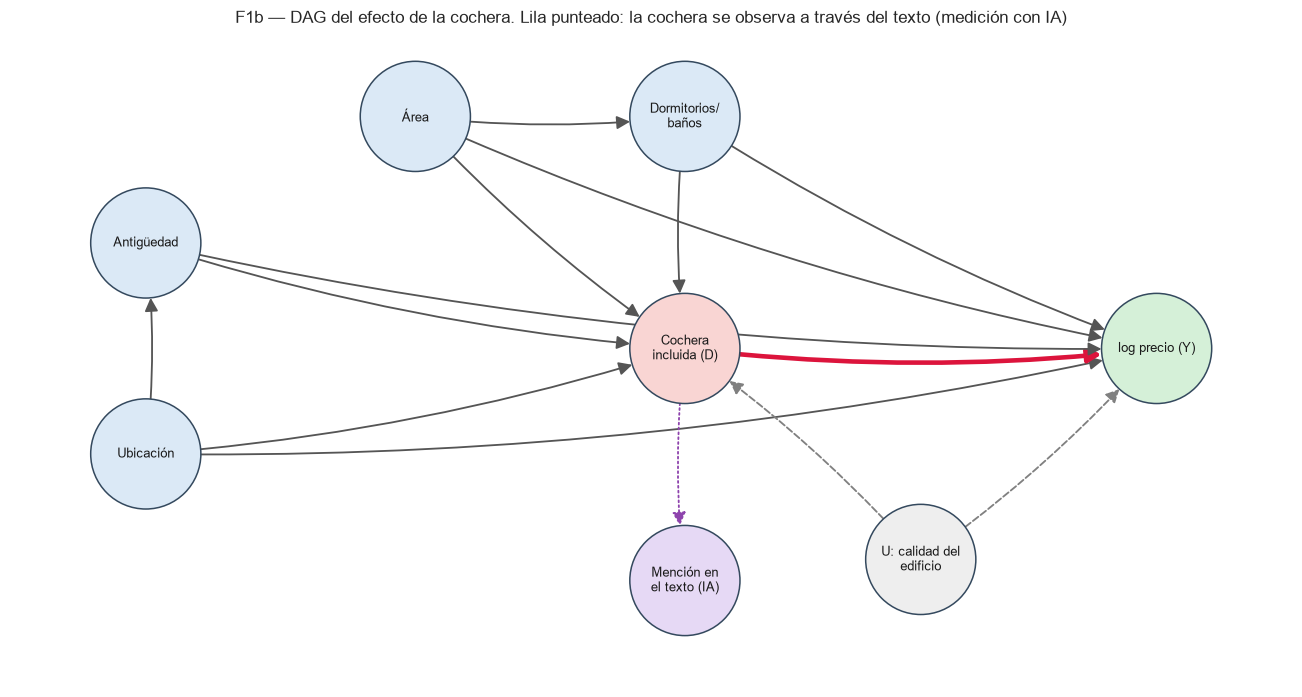
\includegraphics[width=0.95\textwidth]{F1b_dag_cochera.png}
\caption{DAG del efecto de la cochera (F1b). Azul: confusores ajustados; gris punteado: confusor no observado $U$; lila punteado: la cochera se observa a través del texto del aviso.}\label{fig:dag}
\origen{\texttt{notebook3b\_efecto\_cochera.ipynb}, sección 1 $\rightarrow$ \texttt{F1b\_dag\_cochera.png}.}
\end{figure}

La figura~\ref{fig:dag} presenta el modelo causal supuesto, construido con conocimiento del dominio y con el orden temporal de las decisiones. La ubicación y la época de construcción del edificio preceden al diseño. El área, los dormitorios, los baños y la dotación de cocheras se definen en el proyecto. El precio se fija al publicar. Por el criterio \textit{back-door} \citep{pearl2009}, el \textbf{conjunto de ajuste} es: log del área, dormitorios, baños, antigüedad (con un indicador de faltante), latitud, longitud, días publicado, distrito y tipo de lugar devuelto por el geocodificador. El camino $D\leftarrow U\rightarrow Y$ no puede bloquearse con los datos; es la amenaza principal.

Para los baños (análisis secundario) se usa el DAG del entregable anterior (figura~\ref{fig:dag_banos}). Su conjunto de ajuste es el mismo sin los baños; la cochera se agrega como control en una especificación alternativa.

\begin{figure}[H]
\centering
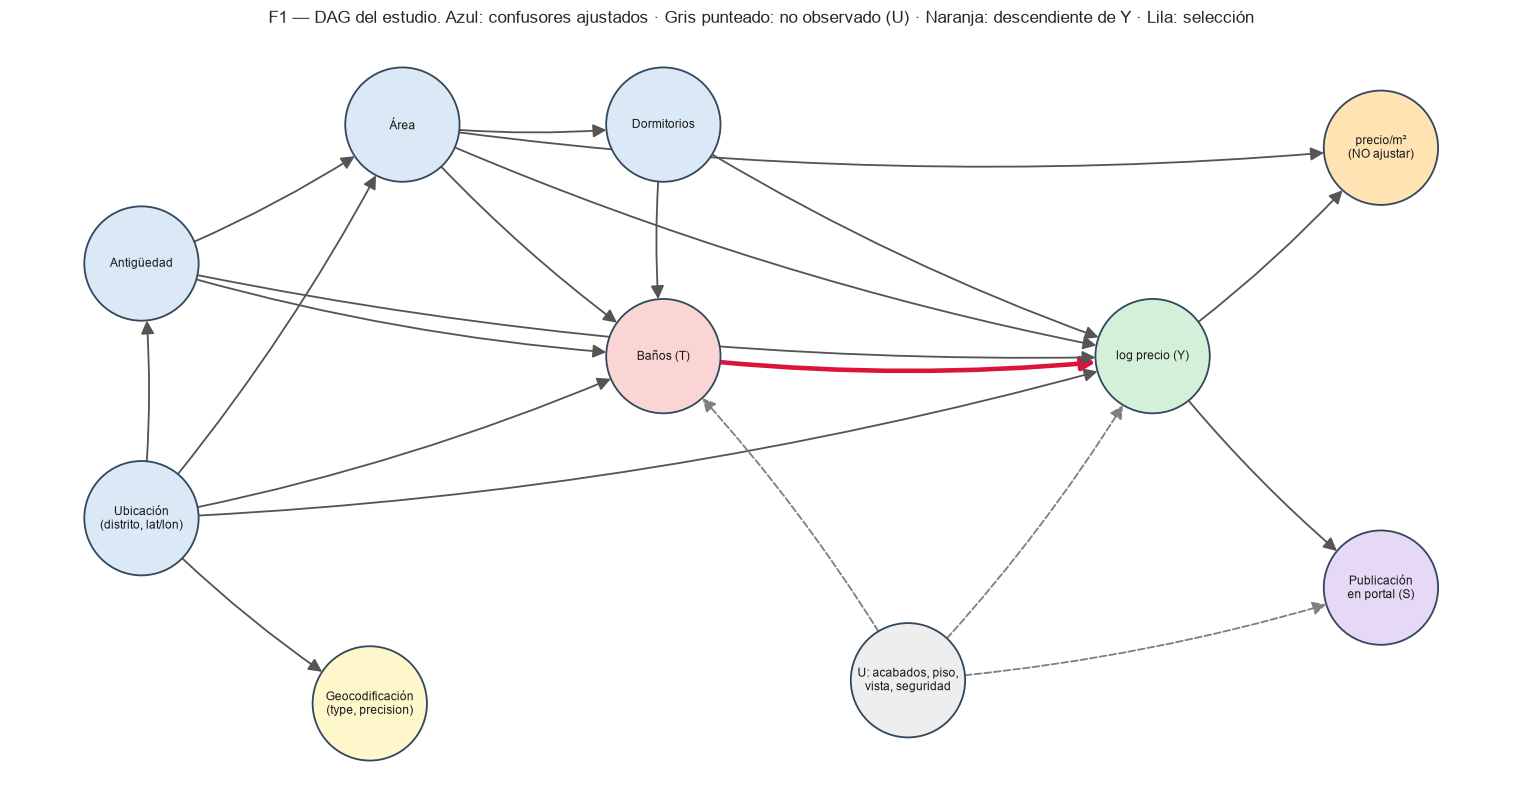
\includegraphics[width=0.85\textwidth]{F1_dag.png}
\caption{DAG del análisis secundario: efecto de un baño adicional (F1).}\label{fig:dag_banos}
\origen{\texttt{notebook3\_estimacion\_causal.ipynb}, sección 1 $\rightarrow$ \texttt{F1\_dag.png}.}
\end{figure}

\section{Papel de cada variable: buenos y malos controles}

\begin{table}[H]
\centering\small
\caption{Papel de cada variable respecto del efecto de la cochera sobre el precio}\label{tab:roles}
\begin{tabularx}{\textwidth}{>{\raggedright\arraybackslash}p{3.0cm}>{\raggedright\arraybackslash}p{2.4cm}>{\raggedright\arraybackslash}p{2.4cm}X}
\toprule
Variable & Papel & ¿Ajustar? & Justificación \\
\midrule
Ubicación (distrito, lat., lon.) & Confusor & Sí & Precede al proyecto; define la escasez de cocheras y el precio \\
Área & Confusor & Sí & Departamentos grandes suelen venir con cochera y cuestan más \\
Baños y dormitorios & Confusores & Sí & Reflejan el estándar del proyecto; no son consecuencia de la cochera \\
Antigüedad & Confusor & Sí & Los edificios antiguos tienen menos cocheras y distinto precio \\
Días publicado, tipo de geocodificación & Previas / artefacto & Sí & Absorben diferencias del aviso y error de ubicación \\
Precio por m² & Descendiente de $Y$ & \textbf{No} & Es el resultado dividido por el área \\
Mención de cochera en el texto & Medición de $D$ & -- & Define el tratamiento; su error es una amenaza \\
Calidad del edificio, amenidades & Confusor no observado $U$ & Imposible & Amenaza principal; se acota con análisis de sensibilidad \\
Publicación en el portal & Selección & Por diseño & Los resultados valen para avisos publicados \\
\bottomrule
\end{tabularx}
\end{table}

\section{Selección, causalidad espacial y amenazas a la validez}

\paragraph{Selección.} La muestra contiene solo departamentos publicados, vigentes en la fecha de captura y con dirección geocodificada con exactitud. Las direcciones exactas son algo más caras y se concentran en los distritos de mayor precio. Por eso los resultados valen para esa población y no se transportan al parque residencial ni a los precios de contrato.

\paragraph{Dependencia espacial.} Departamentos cercanos comparten entorno y los avisos de un mismo edificio comparten su calidad. El \textit{cross-fitting} se agrupa por edificio, los errores estándar se agrupan por edificio (y, como alternativa, por bloques de 1\,km) y la autocorrelación residual se mide con el I de Moran.

\paragraph{Amenazas.} (i) Confusores no observados de calidad. (ii) Error de medición del tratamiento: omisiones en el texto, descripciones truncadas por el portal y errores del modelo de lenguaje. (iii) Duplicados que inflan la precisión. (iv) Reglas de depuración basadas en el precio. (v) Extrapolación fuera del soporte común. Cada una se aborda con una especificación alternativa (capítulo~\ref{cap:diseno}).
